\documentclass[
  11pt,
  twocolumn,
  a4paper,
%  bibliography=totoc,     % Literatur im Inhaltsverzeichnis
]{article}


% Paket float verbessern
\usepackage{scrhack}

% Warnung, falls nochmal kompiliert werden muss
\usepackage[aux]{rerunfilecheck}

% unverzichtbare Mathe-Befehle
\usepackage{amsmath}
% viele Mathe-Symbole
\usepackage{amssymb}
% Erweiterungen für amsmath
\usepackage{mathtools}
% Fonteinstellungen
\usepackage{fontspec}
% Latin Modern Fonts werden automatisch geladen
% Alternativ zum Beispiel:
%\setromanfont{Libertinus Serif}
%\setsansfont{Libertinus Sans}
%\setmonofont{Libertinus Mono}

% Wenn man andere Schriftarten gesetzt hat,
% sollte man das Seiten-Layout neu berechnen lassen
% \recalctypearea{}
% deutsche Spracheinstellungen
\usepackage{polyglossia}
\setmainlanguage{german}

\usepackage{marvosym}
\usepackage[
  math-style=ISO,    % ┐
  bold-style=ISO,    % │
  sans-style=italic, % │ ISO-Standard folgen
  nabla=upright,     % │
  partial=upright,   % ┘
  warnings-off={           % ┐
    mathtools-colon,       % │ unnötige Warnungen ausschalten
    mathtools-overbracket, % │
  },                       % ┘
]{unicode-math}

% traditionelle Fonts für Mathematik
\setmathfont{Latin Modern Math}
% Alternativ zum Beispiel:
%\setmathfont{Libertinus Math}

\setmathfont{XITS Math}[range={scr, bfscr}]
\setmathfont{XITS Math}[range={cal, bfcal}, StylisticSet=1]

% Zahlen und Einheiten
\usepackage[
  locale=DE,                   % deutsche Einstellungen
  separate-uncertainty=true,   % immer Fehler mit \pm
  per-mode=symbol-or-fraction,
  alsoload=hep,                % / in inline math, fraction in display math
]{siunitx}
\sisetup{math-micro=\text{µ},text-micro=µ}
\DeclareSIUnit\micron{\micro\metre}
\DeclareSIUnit\mrad{\milli\rad}
\DeclareSIUnit\gauss{G}
\DeclareSIUnit\eVperc{\eV\per\clight}
\DeclareSIUnit\nanobarn{\nano\barn}
\DeclareSIUnit\picobarn{\pico\barn}
\DeclareSIUnit\femtobarn{\femto\barn}
\DeclareSIUnit\attobarn{\atto\barn}
\DeclareSIUnit\zeptobarn{\zepto\barn}
\DeclareSIUnit\yoctobarn{\yocto\barn}
\DeclareSIUnit\nb{\nano\barn}
\DeclareSIUnit\pb{\pico\barn}
\DeclareSIUnit\fb{\femto\barn}
\DeclareSIUnit\ab{\atto\barn}
\DeclareSIUnit\zb{\zepto\barn}
\DeclareSIUnit\yb{\yocto\barn}

% chemische Formeln
\usepackage[
  version=4,
  math-greek=default, % ┐ mit unicode-math zusammenarbeiten
  text-greek=default, % ┘
]{mhchem}

% richtige Anführungszeichen
\usepackage[autostyle]{csquotes}

% schöne Brüche im Text
\usepackage{xfrac}

% Standardplatzierung für Floats einstellen
\usepackage{float}
\floatplacement{figure}{htbp}
\floatplacement{table}{htbp}

\RequirePackage{luatex85}
\usepackage[
  locale=DE,
]{siunitx}

\usepackage{tikz}
\usepackage[
  europeanresistors, % follow DIN
  americaninductors, % follow DIN
  siunitx,
]{circuitikz}
\usepackage{stackengine}
\AtBeginDocument{
  \sisetup{
    math-rm=\mathrm,
    math-micro=µ, % AltGr+m = MICRO SIGN, Unicode: U+00B5
  }
}

% Floats innerhalb einer Section halten
\usepackage[
  section, % Floats innerhalb der Section halten
  below,   % unterhalb der Section aber auf der selben Seite ist ok
]{placeins}

% Seite drehen für breite Tabellen: landscape Umgebung
\usepackage{pdflscape}

% Captions schöner machen.
\usepackage[
  labelfont=bf,        % Tabelle x: Abbildung y: ist jetzt fett
  font=small,          % Schrift etwas kleiner als Dokument
  width=0.9\textwidth, % maximale Breite einer Caption schmaler
]{caption}
% subfigure, subtable, subref
\usepackage{subcaption}

% Grafiken können eingebunden werden
\usepackage{graphicx}
% größere Variation von Dateinamen möglich
\usepackage{grffile}

% schöne Tabellen
\usepackage{booktabs}

% Verbesserungen am Schriftbild
\usepackage{microtype}

% Literaturverzeichnis
\usepackage[
  backend=biber,
]{biblatex}
% Quellendatenbank
\addbibresource{lit.bib}
\addbibresource{programme.bib}

% Hyperlinks im Dokument
\usepackage[
  unicode,        % Unicode in PDF-Attributen erlauben
  pdfusetitle,    % Titel, Autoren und Datum als PDF-Attribute
  pdfcreator={},  % ┐ PDF-Attribute säubern
  pdfproducer={}, % ┘
]{hyperref}
% erweiterte Bookmarks im PDF
\usepackage{bookmark}

% Trennung von Wörtern mit Strichen
\usepackage[shortcuts]{extdash}

%Multirow Einbindung
\usepackage{multirow}

%rotating Einbindung
\usepackage{rotating}

%noindent immer da


% \documentclass[11pt, twocolumn, a4paper]{article}

\setlength{\oddsidemargin}{0.0 cm}
\setlength{\evensidemargin}{0.0 cm}
\setlength{\topmargin}{-1cm}
\setlength{\textheight}{24 cm}
\setlength{\textwidth}{16 cm}

\pagestyle{plain}

\setlength{\parindent}{0in}

\begin{document}

\author{Nils Breer}

\title{Summary of \textit{Update of the $B^0$ \to $K^{*0}$ µ$^{+}$ µ$^{-}$ angular analysis at LHCb}}

\maketitle
% quick overview what it is about
The stated Process is of such importance because the
$b \to s \mu \mu$ transition is forbidden at tree level due to FCNC.
A study of this is preferebly done with indirect searches because the energy scales can be set much larger than in in direct searches, therefore new Physics(NP)is more accesible.
\begin{figure}
  \centering
  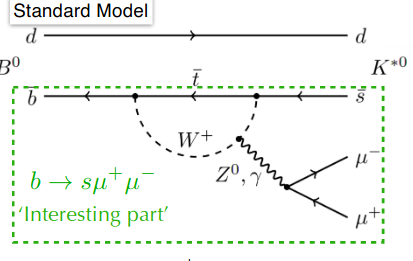
\includegraphics[width=0.5\textwidth]{pictures/sm_flavordiagram.png}
  \caption{Process in standard model.}
  \label{fig:sm_process}
\end{figure}

\begin{figure}
  \centering
  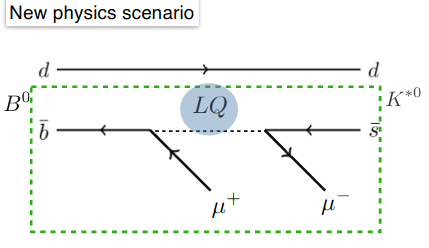
\includegraphics[width=0.5\textwidth]{pictures/NP_flavordiagram.png}
  \caption{Process in new physics model.}
  \label{fig:np_process}
\end{figure}

In figure \ref{fig:np_process}, instead of a suppressed loop via a W-boson which decays weak into a neutral gauge boson and then further into two muons, the NP model suggest a leptoquark as "gauge boson".
Leptoquarks (mostly denoted as X- and Y-Boson) are particles postulate by the GIM model, which provides a way to change a quark into a lepton via the decay channel
\begin{equation*}
  X \rightarrow l^{+} + \bar{\symup{D}}
\end{equation*}

\section{transition in effective theory}
Instead of calculating the well known transition via box diagram, we now factorize out the loops and replace them with an effective coupling (analogous to 4f coupling).
This results in a 4-particle-vertex which is  now described with Wilson coefficents with are sensitive to NP.

With these changes an effective Hamiltonian $H_{eff}$ can be written as
\begin{equation*}
  H_{eff} = - \frac{4 G_f}{\sqrt{2}} \symup{V}_{tb} \symup{V}_ts^{*} \sum_i
  \left( C_i \cdot O_i + C_i\prime \cdot O_i\prime \right)
\end{equation*}
where $C_i$ are the short ranged ilson coefficents which we ant to study. The $O_i$ are the long distance, low energy QCD operators which follow the formfactors.

\section{Angular Analysis}
With the angular analysis we want to measure the decay rate of a process as a function of the final state decay angles, which are schematically shown in figure \ref{fig:angle_1}.

\begin{figure}
  \centering
  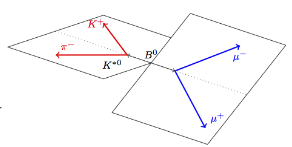
\includegraphics[width=0.5\textwidth]{pictures/angle_1.png}
  \caption{schematical image of decay angles.}
  \label{fig:angle_1}
\end{figure}

The three important angles are $\theta_{k}$, $\theta_{l}$ and $\phi$.
Because the two leptons and the Kaon and Pion are produced in sort of opposite directions, $\theta_{k}$ is the angle between the Kaon and the vector sum of the Kaon and the Pion, which is the general flight direction.
For $\theta_{l}$ it is the same argumentation but for the positive lepton and the fligh direction of the leptons.

In general, the leptons do not fly in the exact same direction, so their dircetion vector span a plane.
This is also true for the Pion and the Kaon.
The angle $\phi$ is the the angle between the normalvector of the K-$\pi$-plane and the $\mu$-$\mu$-plane.
This analysis can give access to more observables with reduced uncertainties.
%
% \section{Early LHCb Measurementsand local tension}
%
%
% \section{Eventselection}
%
%
% \section{Signal and Background}
%
%
% \section{angular fit model vs full fit model}
%
%
% \section{Efficiency}
%
%
% \section{s-wave contribution}
%
%
% \section{Uncertainties}
%
%
% \section{Discussion}
%
%
% \section{Conclusion}


% \printbibliography{}
\end{document}
